

%%%%%%%%%%%%%%%%%%%%%%%%%%%%%%%%%%%%%%%%%

%----------------------------------------------------------------------------------------
%	PACKAGES AND THEMES
%----------------------------------------------------------------------------------------

\documentclass{beamer}

\mode<presentation> {

% The Beamer class comes with a number of default slide themes
% which change the colors and layouts of slides. Below this is a list
% of all the themes, uncomment each in turn to see what they look like.

%\usetheme{default}
%\usetheme{AnnArbor}
%\usetheme{Antibes}
%\usetheme{Bergen}
%\usetheme{Berkeley}
%\usetheme{Berlin}
%\usetheme{Boadilla}
%\usetheme{CambridgeUS}
%\usetheme{Copenhagen}
%\usetheme{Darmstadt}
%\usetheme{Dresden}
%\usetheme{Frankfurt}
%\usetheme{Goettingen}
%\usetheme{Hannover}
%\usetheme{Ilmenau}
%\usetheme{JuanLesPins}
%\usetheme{Luebeck}
\usetheme{Madrid}
%\usetheme{Malmoe}
%\usetheme{Marburg}
%\usetheme{Montpellier}
%\usetheme{PaloAlto}
%\usetheme{Pittsburgh}
%\usetheme{Rochester}
%\usetheme{Singapore}
%\usetheme{Szeged}
%\usetheme{Warsaw}

% As well as themes, the Beamer class has a number of color themes
% for any slide theme. Uncomment each of these in turn to see how it
% changes the colors of your current slide theme.

%\usecolortheme{albatross}
%\usecolortheme{beaver}
%\usecolortheme{beetle}
%\usecolortheme{crane}
%\usecolortheme{dolphin}
%\usecolortheme{dove}
%\usecolortheme{fly}
%\usecolortheme{lily}
%\usecolortheme{orchid}
%\usecolortheme{rose}
%\usecolortheme{seagull}
%\usecolortheme{seahorse}
%\usecolortheme{whale}
%\usecolortheme{wolverine}

%\setbeamertemplate{footline} % To remove the footer line in all slides uncomment this line
%\setbeamertemplate{footline}[page number] % To replace the footer line in all slides with a simple slide count uncomment this line

%\setbeamertemplate{navigation symbols}{} % To remove the navigation symbols from the bottom of all slides uncomment this line
}

\usepackage{graphicx} % Allows including images
\usepackage{booktabs} % Allows the use of \toprule, \midrule and \bottomrule in tables
\usepackage[vietnamese]{babel}
%----------------------------------------------------------------------------------------
%	TITLE PAGE
%----------------------------------------------------------------------------------------

\title[Presentation ]{Đồ án \#1 - Human Parsing \& Pose Estimation
} % The short title appears at the bottom of every slide, the full title is only on the title page

\author{ Đinh Đức Anh Khoa - 23122001 \\ Nguyễn Lê Hoàng Trung - 23122002 \\ Nguyễn Đình Hà Dương - 23122004 \\ Đinh Đức Tài - 23122013
} % 

\institute[23TNT1] % Your institution as it will appear on the bottom of every slide, may be shorthand to save space
{
FIT@HCMUS \\ % Your institution for the title page
\medskip
\textit{TPHCM, tháng 12 năm 2023} % 
}
\date{} % Date, can be changed to a custom date

\begin{document}

\begin{frame}
\titlepage % Print the title page as the first slide
\end{frame}

\begin{frame}
\frametitle{Tổng quan} % Table of contents slide, comment this block out to remove it
\tableofcontents % Throughout your presentation, if you choose to use \section{} and \subsection{} commands, these will automatically be printed on this slide as an overview of your presentation
\end{frame}

%----------------------------------------------------------------------------------------
%	PRESENTATION SLIDES
%----------------------------------------------------------------------------------------
\section{Mở đầu} 
%________________Slide 1__________________
\begin{frame}
\frametitle{1. Mở đầu}
\begin{itemize}
\item Trong bài thuyết trình này, ta sẽ tìm hiểu các khái niệm huấn luyện mô hình học máy, pre-trained model, phương pháp Human Parsing và Pose Estimation

\end{itemize}

\begin{figure}[h]
\centering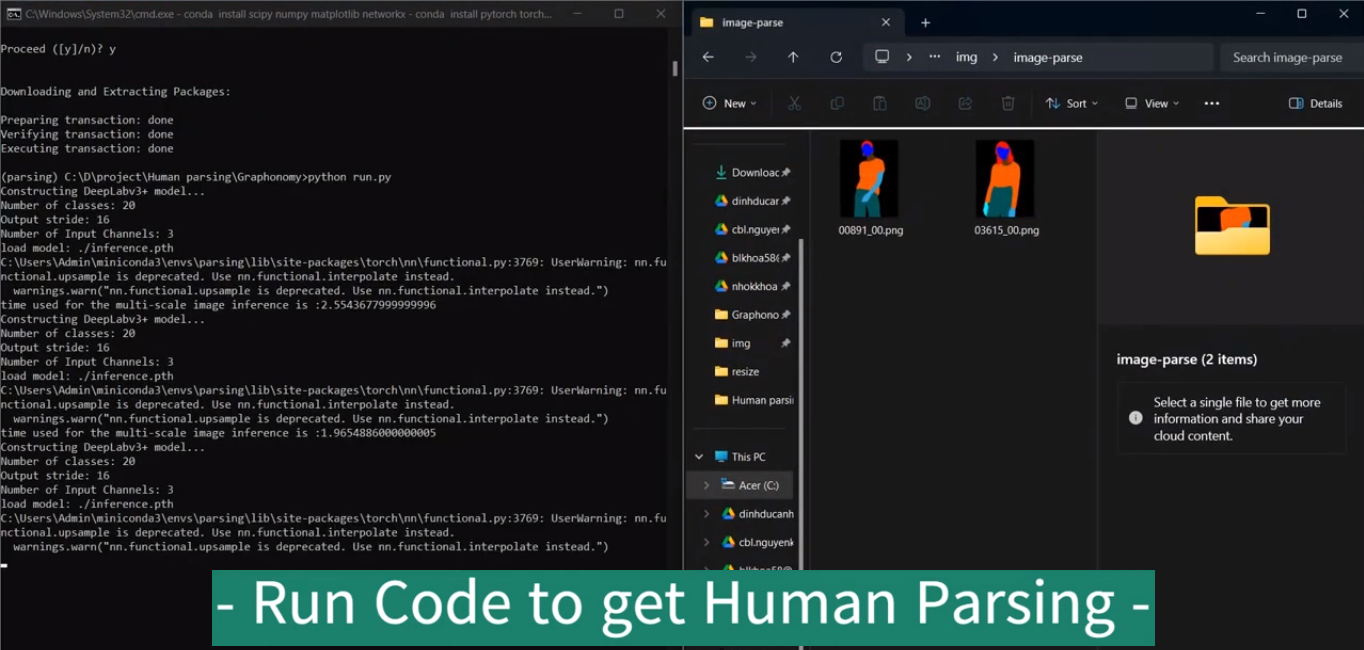
\includegraphics[width=1\linewidth]{images/pic1.png}
\end{figure}

\end{frame}

\begin{frame}

\section{Các khái niệm về học máy - model} 
\frametitle{2. Các khái niệm về học máy - model}

\begin{itemize}
\item Huấn luyện mô hình học máy
\item Pre-trained model

\end{itemize}

\end{frame}

%_______________Silde 1.1____________________

\begin{frame}
\frametitle{2.1 Huấn luyện mô hình học máy}

\begin{block}{Quá trình huấn luyện mô hình học máy}
là quá trình cung cấp dữ liệu đầu vào và đầu ra cho
mô hình, để mô hình có thể học từ dữ liệu và tìm ra một hàm ánh xạ từ dữ liệu đầu vào sang đầu
ra tương ứng. Mô hình được huấn luyện thông qua việc điều chỉnh các tham số (trọng số) của nó
dựa trên sự khác biệt giữa đầu ra thực tế và đầu ra được dự đoán bởi mô hình

\end{block}

\begin{block}{Input, Output}
Input (đầu vào) của mô hình học máy là dữ liệu đầu vào, có thể là ảnh, văn bản, âm thanh, hoặc các dạng dữ liệu khác. Output (đầu ra) của mô hình là dự đoán mà mô hình
tạo ra dựa trên đầu vào. Ví dụ, nếu mô hình được huấn luyện để nhận dạng hình ảnh, đầu vào sẽ là một hình ảnh và đầu ra sẽ là nhãn xác định loại đối tượng trong hình ảnh đó.

\end{block}

\end{frame}

%_______________Slide 1.2_______________________
\begin{frame}
\frametitle{2.1 Huấn luyện mô hình học máy}

Quá trình huấn luyện mô hình học máy thường diễn ra qua các bước sau

\begin{enumerate}
    \item Chuẩn bị dữ liệu: Dữ liệu huấn luyện được chuẩn bị và tiền xử lý để đảm bảo độ chuẩn xác và tính đại diện của nó.
    \item Xây dựng mô hình: Mô hình học máy được xây dựng với kiến trúc và các tham số ban đầu.
    \item Định nghĩa hàm mất mát: Một hàm mất mát được chọn để đo lường sai khác giữa đầu ra dự đoán và đầu ra thực tế.
    \item Tối ưu hóa tham số: Mô hình sử dụng một thuật toán tối ưu (như gradient descent) để điều chỉnh các tham số (trọng số) của mô hình để giảm thiểu hàm mất mát.
    \item Đánh giá mô hình: Mô hình được đánh giá thông qua việc sử dụng dữ liệu kiểm tra hoặc dữ liệu đánh giá độc lập để đo lường hiệu suất của nó.
\end{enumerate}

\end{frame}

%------------------------------------------------

\section{Lý do cần Human Parsing và Pose Estimation} 

\begin{frame}
\frametitle{Lý do cần Human Parsing và Pose Estimation}
\begin{figure}
    \centering
    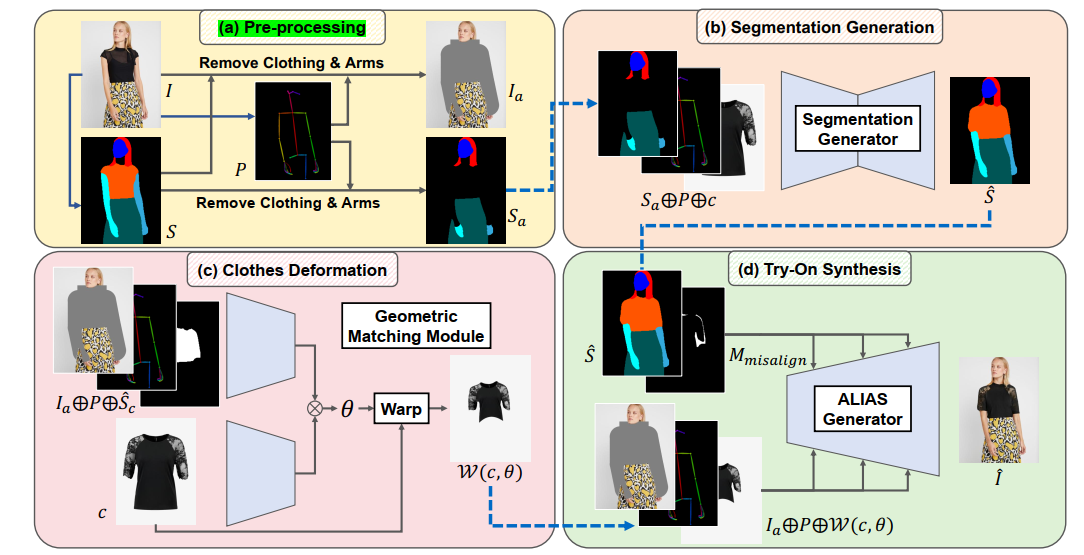
\includegraphics[width=1\linewidth]{image.png}
    
\end{figure}


\end{frame}

\section{Human Parsing} 

\begin{frame}
\frametitle{Human Parsing}

\begin{figure}
    \centering
    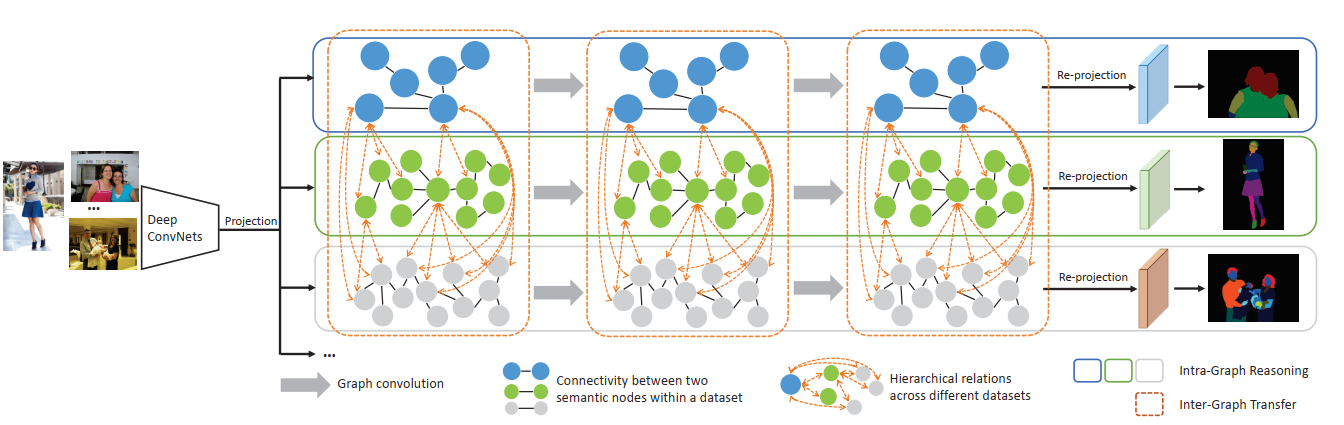
\includegraphics[width=1\linewidth]{p2.png}
    
    
\end{figure}

\end{frame}

\begin{frame}
\frametitle{Human Parsing}

\begin{figure}
    \centering
    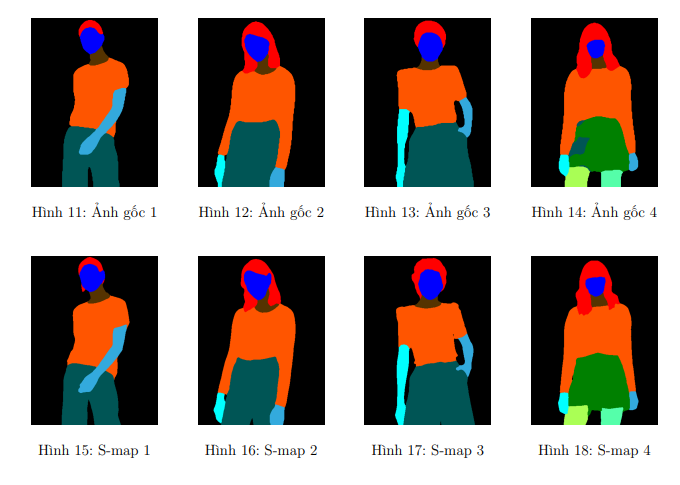
\includegraphics[width=1\linewidth]{p3.png}
    
    
\end{figure}

\end{frame}


\section{Pose Estimation} 


\begin{frame}
\frametitle{Pose Estimation}

\begin{figure}
    \centering
    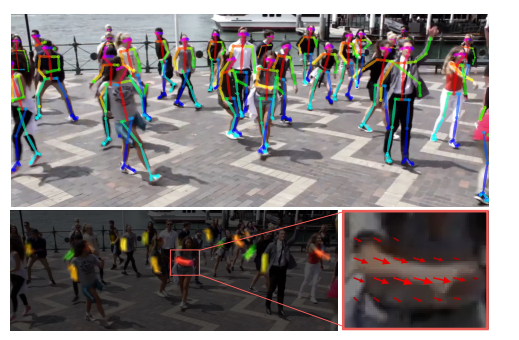
\includegraphics[width=1\linewidth]{p4.png}
    
    
\end{figure}

\end{frame}

\begin{frame}
\frametitle{Pose Estimation}

\begin{figure}
    \centering
    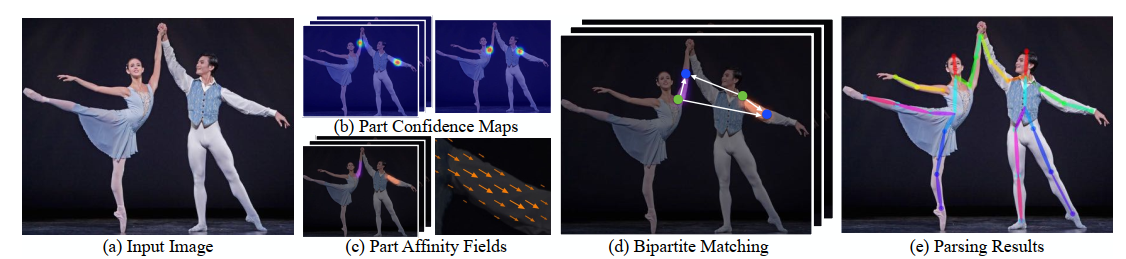
\includegraphics[width=1\linewidth]{p5.png}
    
    
\end{figure}

\end{frame}
\begin{frame}
\frametitle{Pose Estimation}

\begin{figure}
    \centering
    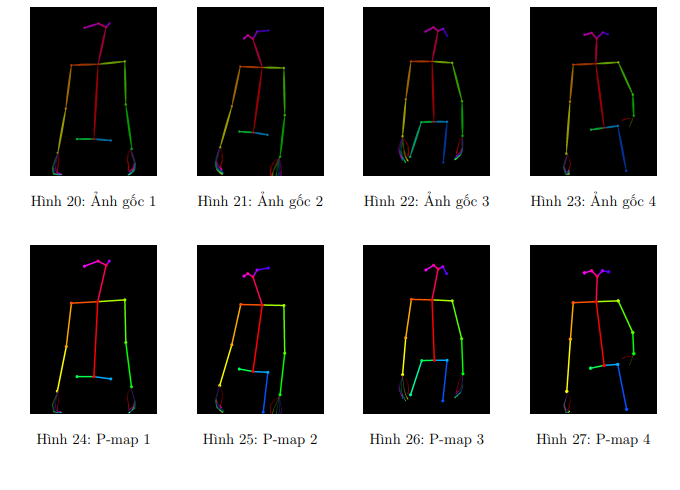
\includegraphics[width=1\linewidth]{p7.png}
    
    
\end{figure}

\end{frame}


%------------------------------------------------
%_________________Slide 6. ______________________
\begin{frame}
\frametitle{Tham Khảo}



\begin{figure}
    \centering
    
\includegraphics[width=0.5\linewidth]{images/qr.png}
\end{figure}


\end{frame}

\begin{frame}
\Huge{\centerline{The End}}
\end{frame}

%----------------------------------------------------------------------------------------

\end{document} 